% $Id: GREIT-algorithm.tex,v 1.21 2008-05-18 14:59:45 aadler Exp $
\documentclass[letterpaper,twocolumn,10pt]{article}
\usepackage[margin=0.75in]{geometry}


\usepackage[compact]{titlesec}
\titlespacing{\section}{0pt}{6pt}{6pt}
\titlespacing{\subsection}{0pt}{6pt}{6pt}

\usepackage{graphicx}
\newcommand{\vB}{\mbox{$\bf v$}}
\newcommand{\xB}{\mbox{$\bf x$}}
\newcommand{\yB}{\mbox{$\bf y$}}
\newcommand{\JB}{\mbox{$\bf J$}}
\newcommand{\RB}{\mbox{$\bf R$}}
\newcommand{\WB}{\mbox{$\bf W$}}
\newcommand{\PB}{\mbox{$\bf P$}}
\newcommand{\MB}{\mbox{$\bf M$}}
\newcommand{\IB}{\mbox{$\bf I$}}
\newcommand{\SG}{\mbox{$\bf \Sigma$}}
\newcommand{\sG}{\mbox{$\bf \sigma$}}
\newcommand{\etal}{{\em et al}}
\begin{document}

\title{\bf GREIT: towards a consensus EIT algorithm for lung images
\normalsize \em (DRAFT: $Date: 2008-05-18 14:59:45 $)%
}

\author{Andy Adler$^{1}$,
        John Arnold$^{2}$,
        Richard Bayford$^{3}$,
        Andrea Borsic$^{4}$,
        Brian Brown$^{5}$,
\\
        Paul Dixon$^{6}$,
        Theo J.C. Faes$^{7}$,
        In\'ez Frerichs$^{8}$,
        Herv\'e Gagnon$^{9}$,
\\
        Yvo G\"arber$^{10}$,
        Bart\l{}omiej Grychtol$^{11}$, 
        William R B Lionheart$^{12}$,
        G\"unter Hahn$^{13}$,
\\
        Anjum Malik$^{14}$,
        Janet Stocks$^{15}$,
        Andrew Tizzard$^{4}$,
        Gerhard Wolf$^{2}$%
       }

\date{}
\maketitle

\renewcommand{\baselinestretch}{0.9} \normalfont

{\small \bf
 {\em Abstract --}
Recently, Electrical Impedance Tomography (EIT) has begun to see a
significant clinical interest for monitoring of
ventilated patients.  The key capability of EIT is to
provide a real-time images of the distribution of ventilation in
the patient's lungs.
However, most clinical and physiological research in lung EIT
is done using older and proprietary algorithms; this is
an obstacle to interpretation of EIT results because the
reconstructed images are not well characterized.
To address this issue, we are developing a
consensus linear reconstruction algorithm for lung EIT,
called GREIT (Graz consensus Reconstruction algorithm for EIT).
This algorithm is being developed in three phases:
1) selection of the ``ingredients'' and evaluation 
methodology (this paper),
2) evaluation and experience with GREIT variants, and
3) consensus and definition of the GREIT algorithm.
Algorithms evaluation criteria are identified to be:
a) quantitative output for all positions,
b) reconstructed position error (low and uniform),
c) resolution (small PSF, uniform, few artefacts),
d) good noise performance,
e) low sensitivity to electrode and boundary movement,
f) good performance on clinical and experimental data.
This approach represents the consensus of a large and representative
group of experts in EIT algorithm and clinical applications.
All software and data to implement and test GREIT will be
made available under an open source license which allows free
research and commercial use.
}

% \noindent{\it Keywords\/}:
% Electrical Impedance Tomography,
% Lung Function Imaging,
% Image Reconstruction,

{\small
 $^{1}$Carleton University, Ottawa, Canada
 $^{2}$Harvard University, Boston, USA
 $^{3}$Middlesex University, London, UK
 $^{4}$Dartmouth College, Hanover, NH, USA
 $^{5}$University of Sheffield, UK
 $^{6}$Cardinal Health Care, London, UK
 $^{7}$Vrije Universiteit, Amsterdam, Netherlands
 $^{8}$University of Kiel, Germany
 $^{9}$\'Ecole Polytechnique de Montr\'eal, Canada
$^{10}$Dr\"ager Medical, L\"ubeck, Germany
$^{11}$University of Strathclyde, Glasgow, UK
$^{12}$University of Manchester, UK
$^{13}$University of G\"ottingen, Germany
$^{14}$Maltron International, Rayleigh, UK
$^{15}$Institute of Child Health, London, UK
}
\renewcommand{\baselinestretch}{1.0} \normalfont


\section{Introduction}
Electrical Impedance Tomography (EIT) measures conductivity
changes within a body from current stimulation and voltage
measurement on the body surface. One of the most promising
applications of EIT is for measuring the lungs, since these
are large organs which undergo large changes in conductivity
during normal functioning. Indeed, lung function measurement
was among the first physiological applications of this technology.
(Barber and Brown 1984).
While there are several medical imaging and instrumentation
technologies to measure ventilation, EIT is unique in that it
is able to non-invasively and continuously monitor the distribution of 
ventilation. Based on these advantages, there is significant
interest in EIT to 
monitor patients with respiratory compromise.

One limitation is that most clinical and physiological research
on lung EIT is being done using proprietary variants of
older image reconstruction algorithms, such as the backprojection
algorithm as implemented
in the Sheffield (Brown and Seagar, 1987)
or G\"ottingen (Hahn \etal, 2001) EIT systems.
This is an obstacle to clinical use of EIT because:
1) it is difficult to determine whether a given image feature is 
physiological or an artefact,
2) comparison of regional ventilation is impacted by
algorithm spatial non-uniformity and position errors,
and 
3) multi-centre studies are not possible without a 
common imaging algorithm.
Many approaches to reconstruct EIT images have been proposed,
however, it is not easy to compare them, because 
complete implementation detail are not available.
However, there is general consensus amongst experts
in EIT image processing of the ``ingredients'' that should
be part of a robust and high performance algorithm.

We plan to address this problem, and to develop a
consensus linear reconstruction algorithm for EIT
images of the chest.
This algorithm is named GREIT, 
the ``Graz consensus Reconstruction algorithm for EIT'',
since early discussions took place at the 2007 EIT conference
in Graz, Austria. Our aim is to develop a standard which
has broad agreement from experts in the mathematical,
engineering, physiological, and clinical EIT communities.
This paper is the first step in developing GREIT:
we define the selection of ``ingredients'' in the
algorithm and the evaluation 
methodology. Subsequently, we plan to evaluate
and gain experience with GREIT ``recipes'' based on 
variants of the ingredients. This will lead to 
consensus and definition of the GREIT algorithm.

The current work is limited to the reconstruction algorithm.
We do not propose calibration tests, data formats or phantoms, standards
for image interpretation or EIT based lung parameters; 
we do not feel there is sufficient experience yet to reach
consensus in these areas.
It is important to clarify that there is no financial
goal to development of this algorithm,
and all developed algorithms, software
models and simulation and experimental test data used
in this algorithm will been made available as part of
the open source EIDORS distribution (Adler and Lionheart, 2006).

The goals identified for GREIT are for:
\begin{list}{$\circ$} %{\textbullet}
  {\leftmargin=1.0em \itemindent=-0.0em
    \topsep=0.0\baselineskip
    \itemsep=-0.4\baselineskip}
\item
 single and double ring electrode
configurations with Sheffield-type EIT systems, using
      adjacent current injection and measurement.
\item
 linear (real-time) reconstruction of a 2D conductivity
change image, based on a 3D forward model
\item
 quantitative reconstructions:
   given an input in transfer impedance ($\Omega$) units,
                    the output is in impedivity change ($\Omega\cdot m$))
\item
 settings for all parameters:
     any tunable parameters must have assigned
     values in the recommended algorithm.
\item
 published reconstruction matrices for
      a $32\times 32$ pixel array for
      for a single ring of $16$, $12$ and $8$ 
      electrodes, for the shapes:
   a) neonate chests, 
   b) adult chests (for perhaps several body shapes), and 
   c) cylindrical tank phantoms.
 For other shapes and electrode configurations,
   reconstruction matrices may be calculated from the
   provided source code.

\item
   all software and data to implement and test GREIT to be
   made available under an open source license which allows 
   royalty free use in both research and commercial applications.

\end{list}


In the remainder of this paper, we clarify two aspects of GREIT:
1) the ``ingredients'' for the algorithm, and
2) the evaluation methodology.

\section{``Ingredients''}

There is general agreement that the algorithm features
described in this section are the most suitable for
linear EIT reconstruction. However, the best selections
for the details of each feature are subject to discussion
and experimentation. For example, we all agree that
regularized image reconstruction techniques are necessary,
but are not yet certain of the best reconstruction matrix prior.
For this reason, we use the metaphor ``ingredients'' and
``recipe''; we are certain of the ingredients, but need
to experiment to find the best recipe.
\begin{figure}[tbh]
\begin{center}
 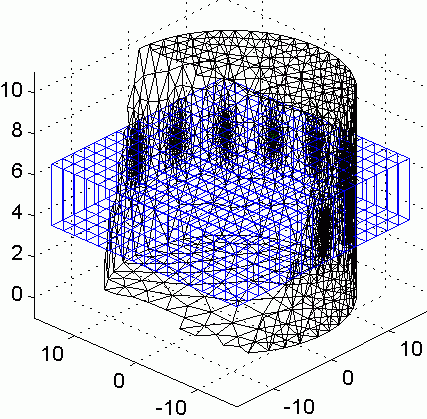
\includegraphics[width= 0.35\textwidth, bb=0 0 427 419]{figs/square_mesh03a.png}
\caption{ \label{fig:dual_model}
\small
Dual model example. {\em black:} a cut away view of a
cylindrical 3D FEM (fine) forward model (with electrode
 refinement),
{\em blue:} (coarse) reconstruction model with 2D square
pixels of defined height.%
\vspace{-0.5cm}
}
\end{center}
\end{figure}

\newcounter{Ictr}
\begin{list}{\bf \arabic{section}.\arabic{Ictr}}
  {\leftmargin=0.0em \itemindent=2.0em
    \topsep= 0.0\baselineskip
    \itemsep=-0.0em
    \listparindent=1.0em \parsep=-0.0em
    \usecounter{Ictr}}

\item {\bf Dual Models}

A dual reconstruction model uses a fine finite element
model (FEM) to implement the forward solution (voltages
at electrodes), and a coarse mesh for the inverse
solution. For GREIT, the forward model is a 3D FEM with
mesh refinement near the electrodes, and the reconstruction
model is square pixel grid (Fig.~\ref{fig:dual_model}).
Given a forward model, $F$,
which calculates a voltage measurement vector, $\vB$, from
a forward (fine) model conductivity element vector, $\sG_f$, we
have $\vB = F( \sG_f )$. The reconstruction (coarse)
model is defined on square elements $\sG_r$ related by
a coarse to fine projection matrix $\PB$, where $\sG_f = \PB \sG_r$.

\item {\bf Rasterized Output image with units}

GREIT output images will be parametrized onto
a 2D grid with square pixels (Fig.~\ref{fig:square_pixels}).
This differs from many EIT reconstruction algorithms
which reconstruct to an arbitrary FEM triangularization.
Square pixels are chosen because it allows easier
display and analysis of images, and because the 
resolution limits of EIT are easier to communicate this way.
Non-circular reconstruction geometries (for adult and
neonate chests) will be represented onto the same 2D grid.

GREIT output images will be in impedivity change units
($\Omega\cdot m$) given input in transfer impedance units
({\em measured V/stimulation I} $=\Omega$). Assigning units
this way requires one length parameter to be measured
from the patient. For GREIT, this is the lateral width of
the chest (or the diameter of the cylindrical tank).

\begin{figure}[tbh]
\begin{center}
 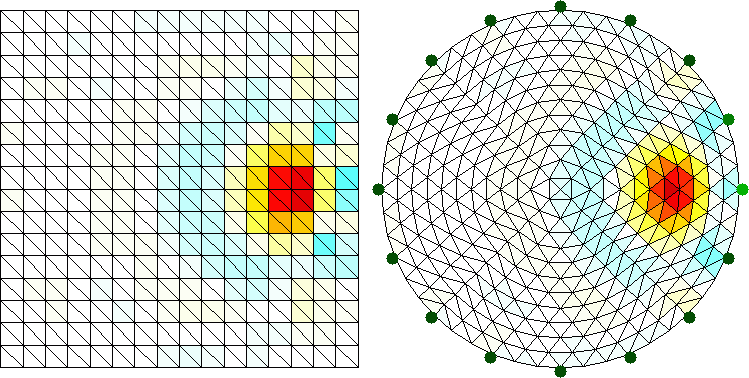
\includegraphics[width= 0.4\textwidth, bb=0 0 749 378]{figs/square_mesh06a.png}
\caption{ \label{fig:square_pixels}
\small
{\em Left}: Reconstructed image onto $16\times 16$ pixel array using
dual model (triangular divisions of pixels is an artefact of EIDORS
representation). Precalculated GREIT models
will use $32\times 32$ pixel array.
{\em Right}: Reconstructed image using a single FEM reconstruction model.
}
\end{center}
\end{figure}

\item {\bf Linearized Regularized Gauss Newton (GN) Reconstruction.}

GN reconstruction seeks a solution $\hat{\xB}$ which minimizes
$$\| \yB - \JB \xB \|^2_{\WB} + \lambda^2\|\xB - \xB_0\|^2_{\RB}.$$
$\yB = \vB^{(b)} - \vB^{(a)}$ is the vector of
time difference measurements (between times $(a)$ and $(b)$).
The choice of times $(a)$ and $(b)$ depend on the measurement
protocol, and often $(a)$ is an average measurement at a time when
the patient physiology is stable (ie end-expiration). The selection
of times $(a)$ and $(b)$ is out of scope for GREIT.
Some groups consider normalized difference measurements
($[\yB]_i = [\vB^{(b)} - \vB^{(a)}]_i / [\vB^{(a)}]_i$), which
has the advantage of compensating for differences between measurement
channels, but makes it difficult to assign units to $\hat{\xB}$. 
Normalized difference measurements will be considered for GREIT.
$\xB = f(\sG^{(b)}_r) - f(\sG^{(a)}_r)$ is the (parametrized) 
conductivity change vector on the inverse model.
The parametrization will be
chosen to maximize the linear range of the solution; 
some possible parametrization functions $f(\cdot)$ are log and linear.

$\JB$ is the Jacobian matrix calculated from the 
fine model and projected on the inverse model,
such that 
$$[\JB]_{ij} = \sum_k \frac{\partial [\yB ]_i}
                           {\partial [ f(\sG_f) - f(\sG_{bkg}) ]_k}
                           \PB_{kj} ,$$ 
where $\sG_{bkg}$ is the background conductivity distribution in 
the body about which conductivity changes take place. Precalculated
GREIT models will assume homogeneous $\sG_{bkg}$, since this
assumption is well understood, even though it is not
physiologically realistic in the chest. Efficient techniques
to compute $\JB$ are out of scope for GREIT, since the calculation
of the Jacobian is off-line.

GN reconstruction uses the 2-norm ($\| \cdot \|^2$), since this
makes image reconstruction linear, and allows precalculation
of a reconstruction matrix. Based on this matrix, real-time
EIT image reconstruction is implemented using matrix multiplication.
It may be possible to increase the computational efficiency
of reconstruction using scaled integer multiplication,
and with use of hardware which supports parallel computation;
however, such implementation details are out of scope for GREIT.

\item {\bf Image Prior with spatial correlations}

$\WB$ and $\RB$ represent the estimates of inverse covariances
of the data noise ($\SG_n$) and conductivity change, or
image prior ($\SG_x$), such that
$\sigma_n^2 \WB^{-1}= \SG_n$ and
$\sigma_x^2 \RB^{-1}= \SG_x$. Here $\lambda= \sigma_n/\sigma_x$,
is the regularization {\em hyperparameter}.
Precalculated GREIT models assume uniform uncorrelated
Gaussian measurement noise, and thus $\WB = \IB$.

Many different approaches have been used to select
the image prior $\RB$, including a scaled diagonal
matrices and various forms of spatial high pass
filters including discrete Laplacian and Gaussian
high pass filters. The choice of $\RB$ has several
subtle but important implications on reconstructed
images, as illustrated in Fig.~\ref{fig:prior_effects}.
We identify these undesirable image features as:
a) {\em ringing:} the presence of opposite polarity
regions surrounding a reconstructed target (which
may be incorrectly interpreted as physiological),
b) {\em position error:} incorrect positioning of
a reconstructed target,
and 
c) {\em blurring:} increased area of a reconstructed
target.
Clearly, there are compromises to be made between
optimizing each features, such as for {\em ringing} and
{\em blurring}. Additionally, the uniformity of
a feature with spatial position is more important
than low average feature errors.

For the evaluation process for GREIT, various
proposed reconstruction matrices (and combinations of
these matrices)
will be tested against the image features. Matrices
will be defined directly on the inverse (coarse) grid
(and not the forward model).


\begin{figure}[tbh]
\begin{center}
 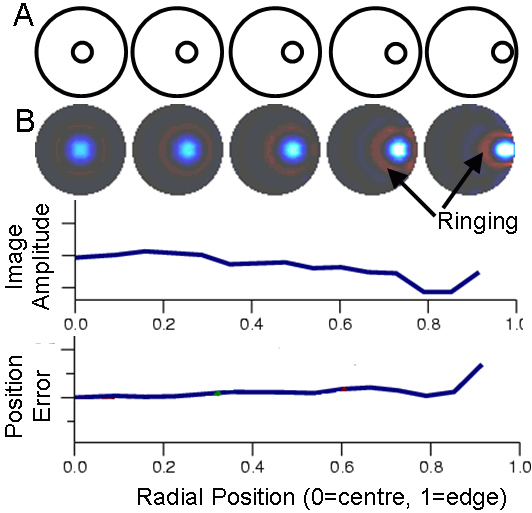
\includegraphics[width= 0.4\textwidth, bb=0 0 512 532]{figs/spatial-uniformity.png}
\caption{ \label{fig:prior_effects}
\small
Illustration of several undesirable features affected by the
choice of $\RB$. {\em A}: Ground truth simulations of a small
non-conductive target. {\em B}: Reconstructed images. The
lower graphs show total image amplitude and position error
as a function of simulated radial position.%
}
\end{center}
\end{figure}

\item {\bf Hyperparameter selection method}

In many studies, the EIT hyperparameter, $\lambda$, is selected
manually based on heuristic criteria, probably because
automatic techniques, such as the L-curve, work poorly
on the EIT problem (Graham and Adler, 2006).  Furthermore,
these methods select the best $\lambda$ for
each image, rather than for the system configuration.

It is essential that GREIT define the hyperparameter 
selection, as this is necessary for reliable
clinical interpretation, or multi-centre studies.
Unfortunately, there is little consensus on the best
way to choose $\lambda$, and thus exploration of 
this issue will be a major part of the GREIT evaluation
process. The criteria for selection are:
$\lambda$ must depend on the EIT equipment (and noise
performance) and the expected EIT signal level (of
thoracic EIT measurements). We propose to define
calibration protocols that may be performed by the 
equipment maker (or as part of installation) from which
an optimal $\lambda$ may be chosen.

\item {\bf Electrode movement and model inaccuracy compensation}

Movement of electrodes due to breathing and posture change
contributes artefacts to EIT images, which appear as
image degradation near the boundary, and a broad artefact
that changes image amplitude. 
Some recent work to correct for movement (Soleimani \etal, 2006)
and general model inaccuracies (Kaipio and Somersalo, 2007)
show promising results and may be represented in a linear
GN reconstruction, by modifying the data noise model
($\SG_n$) to include both measurement noise and ``noise'' 
due to geometrical inaccuracies. Given parameters, $\xB_g$,
which express electrode movement and other model inaccuracies,
we create $\SG_n = \sigma_n^2 \WB^{-1} + \JB_g \RB_g \JB_g^t$,
where $\JB_g$ is the Jacobian of model parameters and $\RB_g$
represents the prior covariance between parameters.

Since such techniques are relatively new, they are less well
understood than the ``ingredients'' discussed previously. 
During the evaluation these techniques may demonstrate
their value, or not.

\item {\bf Temporal reconstruction}

Typically, a frame of EIT data is reconstructed assuming
that all measurements were made at the same movement.
However, EIT systems make sequential measurements for
each current pattern. It is possible to take this
time difference into account to calculate more
accurate EIT images of rapid conductivity changes, such
as those due to perfusion or high frequency oscillatory
ventilation. This approach may be generalized as 
a ``temporal'' image reconstruction (Adler \etal, 2007)
in which measurements from several nearby frames are
used. Such an approach may be used to
achieve improved noise performance.

\end{list}


\section{Evaluation: model data}

This paper also defines the evaluation strategy
against which GREIT algorithms candidates will
be evaluated. Unfortunately, this paper
does not provide space to algorithmically
define how each evaluation parameter is calculated;
instead, the general criteria are listed:

\newcounter{Ectr}
\begin{list}{\bf \arabic{section}.\arabic{Ectr}}
  {\leftmargin=1.0em \itemindent=1.0em
    \topsep= 0.0\baselineskip
    \itemsep=-0.0em
    \listparindent=1.0em \parsep=-0.0em
    \usecounter{Ectr}}

\item {\bf Amplitude Response}
\\ \noindent $\circ$
  output image amplitude is correct
\\ \noindent $\circ$ 
  the amplitude response is uniform for all radial positions.

\item {\bf Position Error}
\\ \noindent $\circ$
  low average position error
\\ \noindent $\circ$
  uniform position error with radial position

\item {\bf Resolution}
\\ \noindent $\circ$
      small average PSF (point spread function) size
\\ \noindent $\circ$
      uniform PSF size with radial position
\\ \noindent $\circ$
      no (or very little) overshoot in the PSF
\\ \noindent $\circ$
      regular shape (round or oval) PSF
  (backprojection, with its streaks, does badly here)

\item {\bf Noise Performance}
\\ \noindent $\circ$
         low average noise amplification

\item {\bf Boundary shape and electrode sensitivity}
\\ \noindent $\circ$
      low sensitivity to electrode movement
\\ \noindent $\circ$
      low sensitivity to boundary distortions
         (with breathing and posture change)

\item {\bf Performance on experimental data}
\\ \noindent $\circ$
 good performance on real experimental animal
    and human clinical images. This includes performance
    monitoring rapid changes with ventilation and perfusion,
    and slow changes over hours and days of monitoring.
    Monitoring of slow changes means that GREIT will need
    to compensate for drift in hardware and electrode
    behaviour.
\end{list}

The most difficult evaluation criteria will be the 
last: ``experimental data performance'' (Faes \etal 2005).
Our approach is based on a database of experimental
EIT data from clinical research groups at Harvard University
and the Universities
of Kiel and G\"ottingen (Hahn \etal, 
2006). Some of these EIT data sets were measured with
simultaneous CT images, which will facilitate developing
validation tests of EIT algorithm output. We also
plan to develop a blinded evaluation protocol for
EIT images.


\section{Discussion}

This paper clarifies two aspects of the
GREIT algorithm: the technical ``ingredients''
and the evaluation methodology. Based on
this description, we aim to select the best
``recipe'' for GREIT algorithm as follows:
First, algorithm candidates will be
built and made available for testing on
simulation and experimental data
(time frame June -- Sept, 2008). 
Based on this experience, a consensus
on each parameter will be developed
and the GREIT algorithm will be
defined and published.
We anticipate several benefits for
this work. It will allow detailed
interpretation of EIT images in terms of
known algorithm performance. This will facilitate
multi-centre EIT tests. For EIT research in
general, it will provide a completely characterized
baseline against which newer work may be compared.



\section*{References}
\renewcommand{\baselinestretch}{0.9} \normalfont {\small

\begin{list}{}
  {\leftmargin=1.0em \itemindent=-1.0em
    \topsep=-1.5\baselineskip
    \itemsep=-0.4\baselineskip}
\item[]
Adler A and Lionheart WRB 2006
``Uses and abuses of EIDORS: An extensible software base for EIT''
{\em Physiol Meas}
27 S25--S42

\item[]
Adler A Dai T Lionheart WRB 2007
``Temporal Image Reconstruction in Electrical Impedance Tomography''
{\em Physiol. Meas.}, 28 S1--S11


\item[]
Barber DC and Brown BH 1984
``Applied potential tomography'', 
{\em J Phys E: Sci Instrum}
 17 723--733
%
%\item[]
%Barber DC 1989
%``A review of image reconstruction techniques for electrical
% impedance tomography''
%{\em Med Phys}
%16 162--169

\item[]
Brown BH and Seagar AD 1987 
``The Sheffield data collection system''
{\em Clin Phys Physiol Meas}
 8(Suppl A) 91--97

\item[]
Cheney M Isaacson D Newell JC Simske S and Goble JC 1990
``NOSER: An algorithm for solving the inverse conductivity problem''
{\em J Imaging Syst Technol} 2 66--75

\item[]
Faes TJC van Genderingen HR and Vonk Noordegraaf A  2006
``Some reflections on the EIT Conference (London UK 22--24 June 2005)''
{\em Physiol. Meas.} 27


%\item[]
%Creative Commons/Science Commons 2007
%``Creative Commons 3.0 Attribution License''
%\verb+creativecommons.org/licenses/by/3.0/+
%
%\item[]
%GNU Lesser General Public License: Version 3, 29 June 2007
%{\em Free Software Foundation, Inc.}
%\verb+www.gnu.org/licenses/lgpl.html+

\item[]
Graham B, Adler A 2006
``Objective selection of the hyperparameter for EIT''
{\em Physiol. Meas.}
27 S65-S79

\item[]
Hahn G Thiel F Dudykevych T Frerichs I Gersing E
and Hellige G 2001
``Quantitative evaluation of the performance of
different electrical tomography devices''
{\em  Biomed Tech (Berlin)}
46 91--95

\item[]
Hahn G Just A Dudykevych T Frerichs I Hinz J Quintel M and Hellige G
2006
``Imaging pathologic pulmonary air and fluid accumulation by functional and absolute EIT''
{\em Physiol. Meas.}
27 S187--S198

\item[]
Kaipio J and Somersalo E 2007
``Statistical inverse problems: Discretization, model reduction and inverse crimes''
{\em J Comput Appl Math}
198 493--504

%\item[]
%Kotre CJ 1988
%``A fast approximation for the calculation of potential distributions in electrical impedance tomography''
%{\em Clin Phys Physiol Meas}
%9 353--361
%
\item[]
Soleimani M G\'omez-Laberge C and Adler A 2006
``Imaging of conductivity changes and electrode movement in EIT''
{\em Physiol. Meas.} 27 S103--S113

\end{list}
} \renewcommand{\baselinestretch}{1.0} \normalfont
\end{document}

